\documentclass{article}

 
% The collection of all the packages I usually require for writing a paper and that are compliant with most Document-Classes

% Required for the right encoding and display of characters
\usepackage[utf8]{inputenc}
\usepackage[T1]{fontenc}
\usepackage[english]{babel}
% Brings colors to your life
\usepackage{color}
%\usepackage[svgnames]{xcolor}
% Math related packages
\usepackage{amsmath}
\usepackage{amsthm}
\usepackage{amssymb}
\usepackage{amsfonts}
\usepackage{mathrsfs}
% additional CS related symbols
\usepackage{stmaryrd}
% Some more missing math features
\usepackage{mathtools}
\usepackage{bbm}
%\usepackage{oz}
% Correct rendering of URLs
\usepackage{url}
% Allows to give custom labels for enum items
\usepackage{enumitem}
% The old but powerful XY package for drawing mostly commutative diagrams
\usepackage[,all,cmtip]{xy}
% Wrapfig allows to have text floating around figures
\usepackage{wrapfig}
% Necessary for \includegraphics command
\usepackage{graphicx}
% The more powerful table package
\usepackage{tabularx}
% Needed for sub-figures
\usepackage{subcaption}
% The free mason pigpen cypher font, that we abuse for pullback and pushout
% pullback is {\pigpenfont J}
% pushout is {\pigpenfont R}
\usepackage{pigpen}
% TiKZ 
\usepackage{tikz}
\usetikzlibrary{cd}
\usetikzlibrary{decorations.pathmorphing}
\usetikzlibrary{shapes,shapes.arrows,shapes.geometric}
\usetikzlibrary{calc}
\usetikzlibrary{positioning}
\pgfdeclarelayer{background}
\pgfdeclarelayer{overlay}
\pgfsetlayers{background,main,overlay}
% Listings
\usepackage{listings}
% Some typographical hacks
%\usepackage{microtype}
% Nicer tables
\usepackage{booktabs}
\usepackage{multirow}
%\usepackage{syntax}
\usepackage{enumitem}




% Macros for writing latex math

\makeatletter

\newcommand{\pto}{}% just for safety
\newcommand{\pgets}{}% just for safety
\DeclareRobustCommand{\pto}{\mathrel{\mathpalette\p@to@gets\to}}
\DeclareRobustCommand{\pgets}{\mathrel{\mathpalette\p@to@gets\gets}}
\newcommand{\p@to@gets}[2]{%
	\ooalign{\hidewidth$\m@th#1\mapstochar\mkern5mu$\hidewidth\cr$\m@th#1\to$\cr}%
}
\makeatother

% Commonly used general concepts
\newcommand{\code}[1]{\texttt{#1}}
\newcommand{\absolute}[1]{\lvert{}{#1}\rvert{}}
\newcommand{\semantics}[1]{\llbracket{}{#1}\rrbracket{}}
\newcommand{\inverse}[1]{{#1}^{-1}}
\newcommand{\dual}[1]{{#1}^{op}}
\newcommand{\kleeneStar}[1]{{#1}^*}
\newcommand{\binprod}[2]{{#1} \times {#2}}
\newcommand{\bincoprod}[2]{{#1} + {#2}}


\newcommand{\rewriteStep}[4]{{#1} \stackrel{{#2}@{#3}}{\rightsquigarrow} {#4}}





% Arrows
\newcommand{\arrow}[3]{{#2}: {#1} \to {#3}}
\newcommand{\inlinearrow}[3]{{#1} \xrightarrow{#2} {#3}}
\newcommand{\longinlinearrow}[3]{\xymatrix{{#1} \ar[r]|{#2} & {#3}}}
\newcommand{\partialarrow}[3]{{#2}: {#1} \rightharpoonup {#3}}
\newcommand{\partialinlinearrow}[3]{{#1} \xrightharpoonup{#2} {#3}}
\newcommand{\partiallonginlinearrow}[3]{\xymatrix{{#1} \ar@{-^{`}}[r]|{#2} & {#3}}}
\newcommand{\relationarrow}[3]{{#2}: {#1} \pto {#3}}
\newcommand{\relationinlinearrow}[3]{{#1} \overset{#2}{\pto} {#3}}
\newcommand{\relationlonginlinearrow}[3]{\xymatrix{{#1} \ar@{-|>}[r]|{#2} & {#3}}}
\newcommand{\inclusionarrow}[3]{{#2}: {#1} \hookrightarrow {#3}}
\newcommand{\inlineinclusionarrow}[3]{{#1} \xhookrightarrow{#2} {#3}}
\newcommand{\longinlininclusionearrow}[3]{\xymatrix{{#1} \ar@{^{(}->}[r]|{#2} & {#3}}}
\newcommand{\monoarrow}[3]{{#2}: {#1} \rightarrowtail {#3}}
\newcommand{\inlinemonoarrow}[3]{{#1} \xrightarrowtail{#2} {#3}}
\newcommand{\longinlinemonoarrow}[3]{\xymatrix{{#1} \ar@{>->}[r]|{#2} & {#3}}}
\newcommand{\epiarrow}[3]{{#2}: {#1} \twoheadrightarrow {#3}}
\newcommand{\inlineepiarrow}[3]{{#1} \xtwoheadrightarrow{#2} {#3}}
\newcommand{\longinlineepiarrow}[3]{\xymatrix{{#1} \ar@{->>}[r]|{#2} & {#3}}}

\newcommand{\worra}[3]{{#2}: {#1} \leftarrow {#3}}
\newcommand{\inlineworra}[3]{{#1} \xleftarrow{#2} {#3}}
\newcommand{\longinlineworra}[3]{\xymatrix{{#1} & {#3} \ar[l]|{#2} }}

\newcommand{\inlinespan}[5]{{#1} \xleftarrow{#2} {#3} \xrightarrow{#4} {#5}}
\newcommand{\inlinecospan}[5]{{#1} \xrightarrow{#2} {#3} \xleftarrow{#4} {#5}}

% Commonly used concepts where notions may have to be tweaked from time to time
\newcommand{\compose}[2]{{#2} \circ {#1}}
\newcommand{\powerset}[1]{\wp{}{#1}}
\newcommand{\identity}[1]{id_{#1}}
\newcommand{\isomorphic}{\cong}
\newcommand{\cat}[1]{\mathbb{#1}}
\newcommand{\functor}[1]{\ensuremath{#1}}
\newcommand{\homset}[3]{{#1}({#2},{#3})}


\newcommand{\catArrows}[1]{\cat{#1}^{\to}}
\newcommand{\catObjects}[1]{\absolute{{#1}}}
\newcommand{\sliceCat}[2]{{#1}\downarrow{}{#2}}
\newcommand{\cosliceCat}[2]{{#1}\uparrow{}{#2}}
\newcommand{\proofStep}[1]{\langle{}\mbox{#1}\rangle{}}


% Adjoints
\newcommand{\leftAdjointTo}[2]{{#1}\dashv{}{#2}}
\newcommand{\unit}[1]{\eta_{#1}}
\newcommand{\counit}[1]{\varepsilon_{#1}}

% Subobject functor
\newcommand{\Sb}[1]{Sub({#1})}
\newcommand{\subob}{\sqsubseteq}
\newcommand{\supob}{\sqsupseteq}
\newcommand{\subobject}[1]{\left[{#1}\right]}
\newcommand{\preimg}[2]{{#1}^{-1}{#2}}
\newcommand{\image}[1]{Im({#1})}


% pullback functor
\newcommand{\pbFunctor}[2]{{#1}^{-1}{#2}}
\newcommand{\upperAdjoint}[2]{\forall_{#1}{#2}}
\newcommand{\lowerAdjoint}[2]{\exists_{#1}{#2}}


% Some functor variables
\newcommand{\F}{\functor{F}}
\newcommand{\G}{\functor{G}}
\newcommand{\U}{\functor{U}}
\renewcommand{\U}{\mathcal{U}}
\newcommand{\Graping}{\Gamma}



% Diagrams

\newcommand{\diagr}[1]{\mathcal{#1}}
\newcommand{\diagrShape}{\cat{S}}


% Partial arrows
\newcommand{\dodef}[1]{dom({#1)}}
\newcommand{\inclPart}[1]{\subseteq_{#1}}
\newcommand{\totalPart}[1]{{#1}}
\newcommand{\inlinespanofpartialMonomap}[5]{
	\xymatrix{{#1} & {#3} \ar@{>->}[l]_{#2}\ar[r]^{#4} & {#5}}
}
\newcommand{\inlinespanofpartialmap}[5]{{#1} \xhookleftarrow{#2} {#3} \xrightarrow{#4} {#5}}
%\newcommand{\inlinespan}[5]{{#1} \xleftarrow{#2} {#3} \xrightarrow{#4} {#5}}
%\newcommand{\inlinecospan}[5]{{#1} \xrightarrow{#2} {#3} \xleftarrow{#4} {#5}}
\newcommand{\partArrName}[2]{[{#1},{#2}\rangle}
%\newcommand{\partialarrow}[3]{{#2}: {#1} \rightharpoonup {#3}}
\newcommand{\subobjClass}[1]{[#1]}
\newcommand{\subobjLessEq}{\sqsubseteq}
\newcommand{\subobjMeet}{\sqcap}
\newcommand{\subobjJoin}{\sqcup}
\newcommand{\subobjBigJoin}{\bigsqcup}

\newcommand{\inlinepartialarrow}[3]{{#1} \xrightharpoonup{#2} {#3}}

% Category of all Sets and functions
\newcommand{\catSet}{\mathbb{S}\mathbb{E}\mathbb{T}}
% Category of all small Categories and morphisms
\newcommand{\catCat}{\mathbb{C}\mathbb{A}\mathbb{T}}
% Category of partial graphs
\newcommand{\relCat}[1]{\code{Rel}(#1)}
\newcommand{\parCat}[1]{\code{Par}(#1)}
\newcommand{\spanCat}[1]{\code{Span}(#1)}
\newcommand{\algCat}[1]{\code{Alg}(#1)}


% Cat of comprehensive systems
\newcommand{\CS}{\cat{C}\cat{S}}
\newcommand{\RCS}{\cat{R}\cat{C}\cat{S}}
\newcommand{\TRCS}[1]{\cat{T}\cat{R}\cat{C}\cat{S}({#1})}
\newcommand{\catBase}{\cat{B}}
\newcommand{\catSchema}{\cat{I}}
\newcommand{\cs}[1]{\mathbf{#1}}
\newcommand{\csLoopVar}{j}
\newcommand{\csLoopVarAll}{i}
\newcommand{\csArrow}[3]{\mathbf{\arrow{#1}{#2}{#3}}}
\newcommand{\csArrowDouble}[3]{\mathbf{\arrow{#1}{#2}{#3}}}
\newcommand{\csWitns}[1]{{#1}^{0}}
\newcommand{\csProj}[2]{\lowercase{#1}^{#2}}
\newcommand{\csProjForall}[1]{\lowercase{#1}^{\csLoopVar}}
\newcommand{\csProjDom}[2]{\dodef{\lowercase{#1}^{#2}}}
\newcommand{\csProjDomForall}[1]{\dodef{\lowercase{#1}^{\csLoopVar}}}
\newcommand{\csProjIncl}[2]{\inclPart{\lowercase{#1}^{#2}}}
\newcommand{\csProjInclForall}[1]{\inclPart{\lowercase{#1}^{\csLoopVar}}}
\newcommand{\csProjTotal}[2]{\totalPart{\lowercase{#1}^{#2}}}
\newcommand{\csProjTotalForall}[1]{\totalPart{\lowercase{#1}^{\csLoopVar}}}
\newcommand{\csCmpnt}[2]{{#1}^{#2}}
\newcommand{\csCmpntForall}[1]{{#1}^{\csLoopVar}}
\newcommand{\csArrOnWtns}[1]{{#1}_0}
\newcommand{\csArrOnCmpnt}[2]{{#1}_{#2}}
\newcommand{\csArrOnCmpntForall}[1]{{#1}_{\csLoopVar}}
\newcommand{\csArrOnDodef}[2]{{#1}_{-{#2}}}
\newcommand{\csArrOnDodefForall}[1]{{#1}_{-{\csLoopVar}}}
%Paper specific
\newcommand{\specialmonos}{\mathscr{M}}
\newcommand{\specialmonoarrow}[3]{\xymatrix{{#1} \ar@{(->}[r]|{#2} & {#3}}}








% All the macros for creating Defitions, Theorems, Proposition etc.
\newtheorem{theorem}{Theorem}
\newtheorem{proposition}{Proposition}
\newtheorem{myfact}{Fact}
\newtheorem{myconj}{Conjecture}
\newtheorem{lemma}{Lemma}
\newtheorem{myclaim}{Claim}
\newtheorem{corollary}{Corollary}
\newtheorem{myparadox}{Paradox}


\theoremstyle{definition}
\newtheorem{definition}{Definition}
\newtheorem{counterexmpl}{Counterexample}
\newtheorem{myaxiom}{Axiom}
\newtheorem{myprinc}{Principle}
\newtheorem{myobs}{Observation}
\newtheorem{myreq}{Requirement}


\theoremstyle{remark}
\newtheorem{myexampl}{Example}
\newtheorem{myremark}{Remark}
\newtheorem{myconv}{Convention}
\newtheorem{myexerc}{Exercise}


\newcommand{\mkTheorem}[3]{
	\begin{mytheo}[{#1}]
	\label{#2}
	{#3}
	\end{mytheo}
}

\newcommand{\mkProposition}[3]{
	\begin{myprop}[{#1}]
		\label{#2}
		{#3}
	\end{myprop}
}

\newcommand{\mkFact}[3]{
	\begin{myfact}[{#1}]
		\label{#2}
		{#3}
	\end{myfact}
}

\newcommand{\mkConjecture}[3]{
	\begin{myconj}[{#1}]
		\label{#2}
		{#3}
	\end{myconj}
}

\newcommand{\mkLemma}[3]{
	\begin{mylemma}[{#1}]
		\label{#2}
		{#3}
	\end{mylemma}
}

\newcommand{\mkClaim}[3]{
	\begin{myclaim}[{#1}]
		\label{#2}
		{#3}
	\end{myclaim}
}
\newcommand{\mkCorollary}[3]{
	\begin{mycorr}[{#1}]
		\label{#2}
		{#3}
	\end{mycorr}
}
\newcommand{\mkParadox}[3]{
	\begin{myparadox}[{#1}]
		\label{#2}
		{#3}
	\end{myparadox}
}


\newcommand{\mkDefinition}[3]{
	\begin{mydef}[{#1}]
	\label{#2}
	{#3}
	\end{mydef}
}

\newcommand{\mkAxiom}[3]{
	\begin{myaxiom}[{#1}]
		\label{#2}
		{#3}
	\end{myaxiom}
}

\newcommand{\mkPrinciple}[3]{
	\begin{myprinc}[{#1}]
		\label{#2}
		{#3}
	\end{myprinc}
}

\newcommand{\mkObservation}[3]{
	\begin{myobs}[{#1}]
		\label{#2}
		{#3}
	\end{myobs}
}

\newcommand{\mkRequirement}[3]{
	\begin{myreq}[{#1}]
		\label{#2}
		{#3}
	\end{myreq}
}

\newcommand{\mkExample}[3]{
	\begin{myexampl}[{#1}]
		\label{#2}
		{#3}
	\end{myexampl}
}

\newcommand{\mkRemark}[3]{
	\begin{myremark}[{#1}]
		\label{#2}
		{#3}
	\end{myremark}
}

\newcommand{\mkConvention}[3]{
	\begin{myconv}[{#1}]
		\label{#2}
		{#3}
	\end{myconv}
}

\newcommand{\mkExercise}[3]{
	\begin{myexerc}[{#1}]
		\label{#2}
		{#3}
	\end{myexerc}
}






\title{Model Transformation - Exercises}
\author{}
\date{}






\begin{document}
	
	\maketitle
	
	\section*{Exercise 1: Miscellaneous}
	
	\begin{enumerate}
		\item Find more examples of model-to-text and model-to-model transformations from your previous developer/student experience. 
		Classify them along the dimensions:
		\begin{itemize}
			\item in-place vs. out-place
			\item homogenous vs. heterogeneous
			\item declarative or imperative
		\end{itemize}
		\item Would you consider the different components of a compiler (lexer, parser, optimizer, code generator, see also Fig.~\ref{fig:compilerPipeline}) as model transformations? Why or why not? 
	\end{enumerate}
	
	\begin{figure}[hbt]
		\centering
		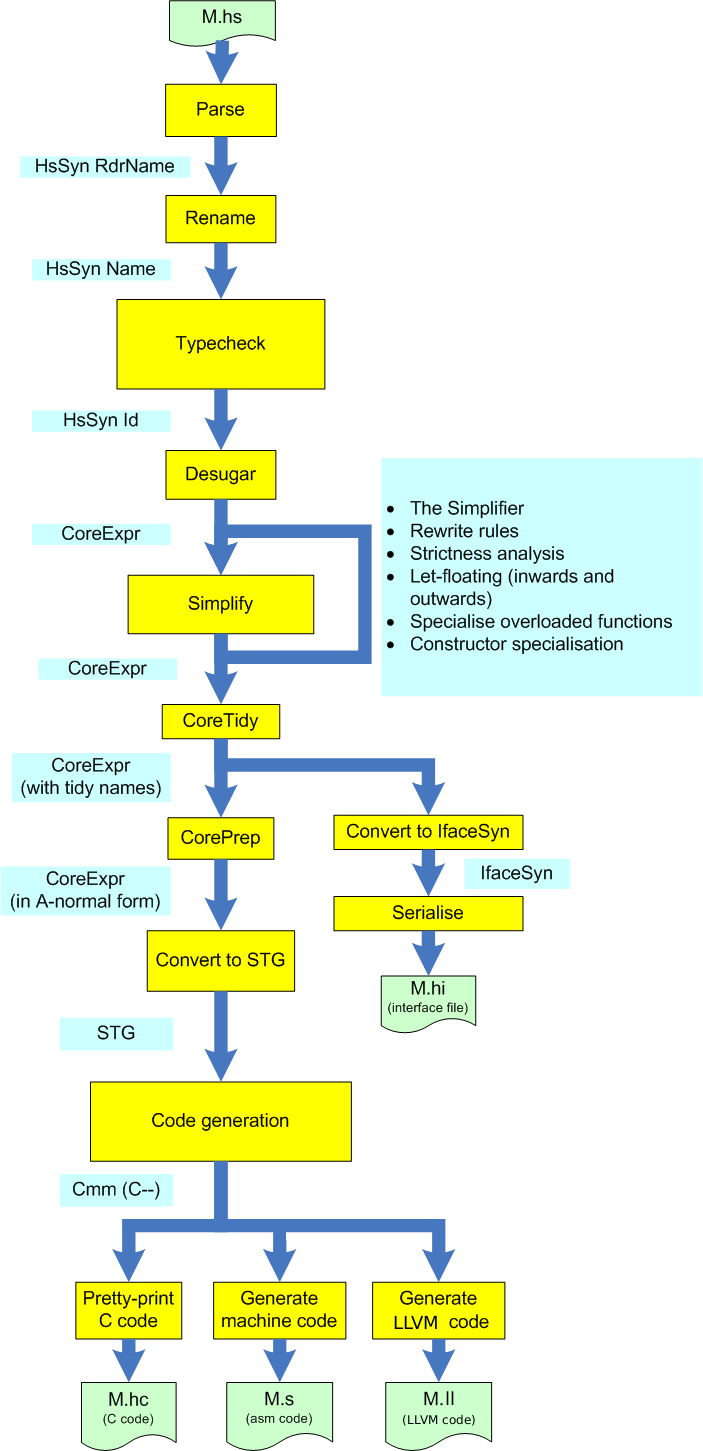
\includegraphics[width=0.32\linewidth]{figures/haskell-pipeline}
		\caption{Haskell compiler pipeline}
		\label{fig:compilerPipeline}
	\end{figure}
	
	\clearpage
	
	\section*{Exercise 2: Blog generator (m2t)}
	
	In this exercise, your task is to write a model-to-text transformation with EGL that provides a \emph{web blog} generation functionality similar to tools like e.g. \emph{Jekyll}\footnote{\url{https://jekyllrb.com/}}.
	The blog content is abstractly defined in a \emph{BLOg Description Language (BLODL)} (Fig.~\ref{fig:blogDSL}, which is defined by the metamodel in Fig.~\ref{fig:blogDSLMetampdel}.
	The resulting file structure (Fig.~\ref{fig:fileStructure}) should contain a folder for each blog \emph{post} containing the respective \emph{html} file and referenced \emph{images}\footnote{This will require you to copy files. For this recall that you can write EOL statements in EGX-scripts, which again allows to call arbitrary Java methods.}.
	The root should contain an html file with hyperlinks to all blog posts.
	Feel free to also add your own custom CSS styles into the generation.
	
	
	\begin{figure}[bth]
		\centering
		\begin{subfigure}[c]{\linewidth}
				\centering
			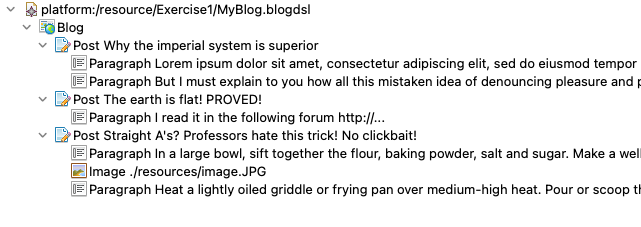
\includegraphics[width=\linewidth]{figures/blog-dsl}
			\caption{Blog DSL}
			\label{fig:blogDSL}
		\end{subfigure}
		\begin{subfigure}[c]{0.5\linewidth}
					\centering
			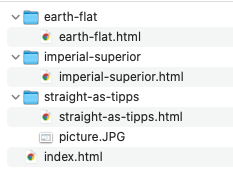
\includegraphics[width=\linewidth]{figures/file-structure}
			\caption{Resulting File Structure}
			\label{fig:fileStructure}
		\end{subfigure}
		\begin{subfigure}[c]{0.45\linewidth}
					\centering
		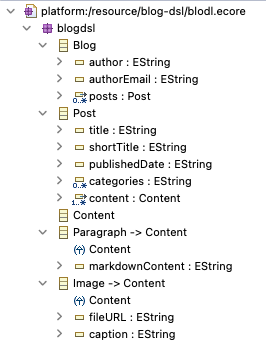
\includegraphics[width=\linewidth]{figures/blog-dsl-metamodel}
		\caption{Blog DSL Metamodel}
		\label{fig:blogDSLMetampdel}
	\end{subfigure}
	\end{figure}
	
	\clearpage
	
	\section*{Exercise 3: Object-Relational-Mapping (m2m)}
	
	In this exercise, your task is to write a model-to-model transformation using ETL that performs an object-relational mapping between \texttt{Ecore} and the relational model \cite{Codd1970}.
	Recall that an \texttt{.ecore} model is yet another model that is typed over the \texttt{Ecore} metamodel.
	An excerpt of the relevant concepts is shown in Fig.~\ref{fig:ecore} (You do not need to consider methods and other more technical details.).
	To find the complete definition of the Ecore metamodel, open the \emph{Plug-in Dependencies} of any project in the \texttt{metamodel-ws} workspace and then navigate to \emph{org.eclipse.emf.ecore\_...} $\rightarrow$ \emph{model} 	$\rightarrow$ \texttt{Ecore.ecore}.
	A metamodel of the relational model, that we are using in this exercise is found in \texttt{metamodel-ws/relational-model/relational.ecore}.
	
	\begin{figure}[htb]
		\centering
		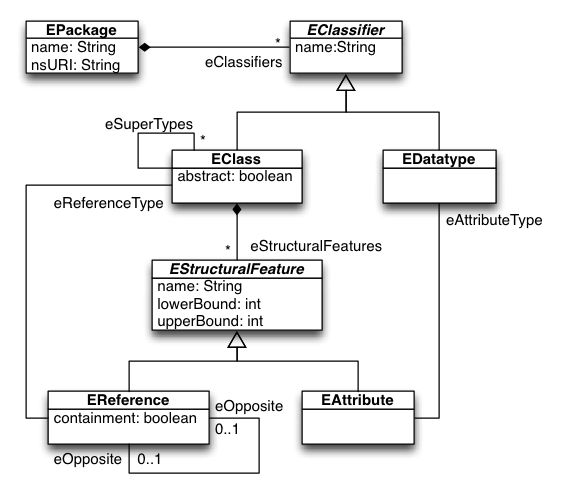
\includegraphics[width=0.7\linewidth]{figures/ecore}
		\caption{Ecore metamodel (simplified)}
		\label{fig:ecore}
	\end{figure}
	
	It is recommended to study both metamodels carefully before you begin and develop your solution step-wise.
	
	
	\begin{enumerate}
		\item Start with a \texttt{Schema} for every \texttt{EPackage} and for every \texttt{EClass} in the package you generate a corresponding \texttt{Table} that contains a single numeric \emph{id} \texttt{Column} with a \texttt{PrimaryKey} constraint on it. 
		The name of the \texttt{Table} should correspond to the \texttt{EClass}, i.e. identical, capitalized or etc.
		
		\item In the next iteration, create a \texttt{Column} in each \texttt{Table} for every \texttt{EAttribute} of the corresponding \texttt{EClass}\footnote{You may require to use the ETL-method \texttt{equivalent()} here}. 
		\texttt{EDataType}s translate as follows:
		\begin{itemize}
			\item \texttt{EString} $\rightarrow$ \texttt{Varchar(4000)}
			\item \texttt{ELong/EInteger,EShort,EByte} $\rightarrow$ \texttt{Number(32,0)}
			\item \texttt{EFloat/EDoubke} $\rightarrow$ \texttt{Number(32,4)}
			\item \texttt{EBoolean} $\rightarrow$ \texttt{Number(1,0)}
			\item \texttt{EEnum} $\rightarrow$ \texttt{Number(2,0)}
		\end{itemize}
		
		
		\item In the third iteration, the task is to translate \texttt{EReference}s to \texttt{ForeignKey}s.
		Here, you have to pay attention to multiplicities:
		A many-to-one relation from a table/class $A$ to table/class $B$ is realized by adding a new numeric column to $A$ that has a foreign key to the primary key of $B$.
		Many-to-many relations, require to create a new \emph{junction} table with two columns pointing with foreign keys to the respective primary keys of $A$ and $B$.
		
		\item In the final iteration,  inheritance must be handled. 
		Implement all three strategies \cite{Fowler2012}
		\begin{itemize}
			\item Single Table Inheritance (table per inheritance hierarchy)\footnote{\url{https://martinfowler.com/eaaCatalog/singleTableInheritance.html}},
			\item Class Table Inheritance (table per class)\footnote{\url{https://martinfowler.com/eaaCatalog/classTableInheritance.html}},
			\item Concrete Table Inheritance (table per concrete class)\footnote{\url{https://martinfowler.com/eaaCatalog/concreteTableInheritance.html}}.
		\end{itemize}
		and design a mechanism such that the user can configure which inheritance mapping strategy should be used\footnote{There are many possibilities, one may chose to use \texttt{EAnnotation}s, an external configuration file etc.}.
		
		
	\end{enumerate}
	
	\clearpage
	
	\section*{Exercise 4: Bidirectional Transformations}
	
	\begin{enumerate}
		\item Let $A$ and $B$ be two models where $A$ has $5$ and $B$ has $4$ elements.
		What is the maximum number of elements in the trace-model \cite{DrivalosKolovosPF2009} of a transformation between $A$ and $B$ if we assume that there cannot be two trace-links referring to the same pair of objects taken from an $A$ and $B$?
		\item Below, you will find a list of transformations. For each case you will have to decide in what direction which can define a \textsc{Get} (derivation) and in which direction you require \textsc{Put} (back propagation).
		Maybe it is also sometime possible to define a \textsc{Get} in both directions or you even require a \textsc{Put} in both directions?
		If you require a \textsc{Put}, clearly state \emph{what} additional information you require from the \emph{source}.
		\begin{itemize}
			\item pairs of numbers \texttt{(Int,Int)} $\leftrightarrow$ their sum \texttt{(Int)}
			\item \texttt{Person} entities with \texttt{givenName} and \texttt{familyName} fields $\leftrightarrow$ \texttt{Person} entities with \texttt{name} fields.
			\item sets \{unordered,unique\} $\leftrightarrow$ lists \{ordered,non-unique\}
			\item an \texttt{Ecore} model $\leftrightarrow$ an XSD file
			\item java classes $\leftrightarrow$ database schema
			\item state machines $\leftrightarrow$ hierarchical state machines
			\item C-code $\leftrightarrow$ Python-code
		\end{itemize}
	\end{enumerate}

\bibliographystyle{plain}
\bibliography{library.bib}
\end{document}